\begin{figure}[!t]
    \centering
    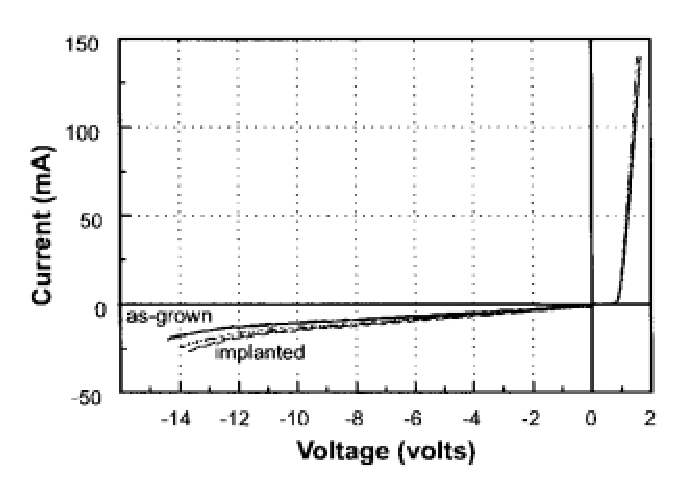
\includegraphics[width=2.5in]{fig/iv}
    \caption{I-V characteristics of p-i-n diodes made from as-grown and blue-shift materials}
    \label{ex_iv}
\end{figure}
For the Ar plasma-induced QWI process to be a useful technique for
lateral bandgap control in monolithic integration, it is essential
that the electrical characteristics of the p-i-n structure not be
degraded by the Ar plasma and/or anneal. Figure llll shows the
current versus voltage (I-V) characteristics for the as-grown and
blue-shift materials following a 120-s RTA at 750 $^\circ$C. We see
that all samples have very similar I-V characteristics.
